\documentclass[conference]{IEEEtran}
\IEEEoverridecommandlockouts
\usepackage{cite}
\usepackage[utf8]{inputenc}
\usepackage[english]{babel}
\usepackage{bookmark}
\usepackage[square,sort,comma,numbers]{natbib}
\usepackage{listings}
\usepackage{url}
\usepackage{wrapfig}
\usepackage{caption}
\usepackage{color}
\usepackage{enumitem}
\usepackage{graphicx}
\usepackage{float}
\usepackage{url}
\def\UrlBreaks{\do\/\do-}
\usepackage{breakurl}
\graphicspath{{images/}}
\usepackage{hyperref}

\def\BibTeX{{\rm B\kern-.05em{\sc i\kern-.025em b}\kern-.08em
    T\kern-.1667em\lower.7ex\hbox{E}\kern-.125emX}}

\begin{document} 
    \title{
        Assignment 4\\[0.3cm]
        \large  Autoencoders/LSTM networks\\
        ELE494-09
    }

    \author{
        \IEEEauthorblockN{Nasir Khalid}
        \IEEEauthorblockA{b00065082\\}
    }

    \maketitle

    \section{Autoencoders and dimensionality reduction}

    We use the fashion MNIST dataset and train a densely connected autoencoder with one hidden layer.
    First with 32 nodes and 64 nodes in this layer with a rectified linear unit as the activation function.
    In the output layer I have a sigmoid activation function. We then train the autoencoder under
    squared error reconstruction loss function. Then I test the networks with the images in the testing
    data, reporting the average reconstruction error for different number of nodes in the hidden layer.
    We then repeat the same with autoencoders with three hidden layers use 32 and 64 as the
    dimensionality of the codes

    \subsection{Preprocessing}

    The data was first imported using Keras and the dimensions of the training/test data were as follows:
    \begin{itemize}
        \item Size of Training Images is (60000, 784)
        \item Size of Test Images is (10000, 784)
    \end{itemize} 
    The pixel values were then normalized between 0 and 1. Shown below is a sample image from
    the Fashion MNIST dataset.

    \begin{figure}[H]
        \centering
        \captionsetup{justification=centering}
        \centering
            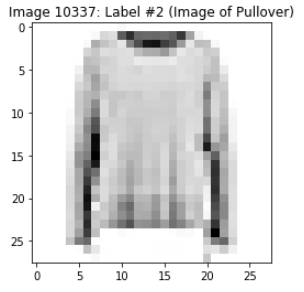
\includegraphics[width=0.15\textwidth]{1.png}
            \caption{Fashion MNIST sample image}
    \end{figure}

    A function was also defined for the average reconstruction error and this function was then 
    passed as a metric in to the networks compile method, this way the average reconstruction error
    was returned on every training epoch. It was defined as follows:

    \begin{equation}
        \frac{1}{Length} \sum |Output - Prediction|
    \end{equation}

    Where Length is the output length, Output is label output and prediction is result of forward pass.
    
% ---------------------------------------------------- Encoder with 1 Hidden Layer that has 32 Nodes --------------------------------------------------------------------------------------------------------
    \subsection{Training Encoder with 1 Hidden Layer that has 32 Nodes}

    Shown below is the summary of the Encoder created with 1 Hidden Layer that has 32 Nodes

    \begin{figure}[H]
        \centering
        \captionsetup{justification=centering}
        \centering
            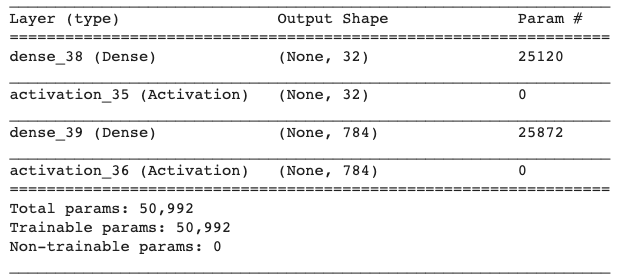
\includegraphics[width=0.45\textwidth]{Encoder_1_32.png}
            \caption{Summary of Encoder with 1 Hidden layer with 32 Nodes}
    \end{figure}

    This encoder was trained up 50 epochs and in the end these were it's final metrics:

    \begin{itemize}
        \item Loss: 0.0128
        \item Average Reconstruction Error: 0.0644
        \item Validation Loss: 0.0130
        \item Validation Average Reconstruction Error: 0.0650
    \end{itemize}

    Shown below is the Epochs vs Loss curve for the network:

    \begin{figure}[H]
        \centering
        \captionsetup{justification=centering}
        \centering
            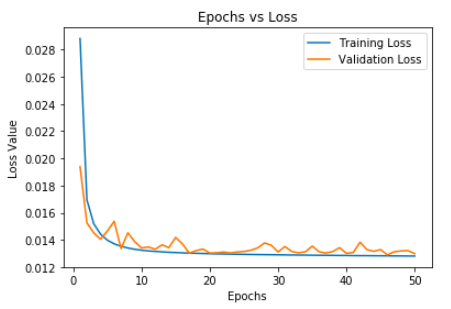
\includegraphics[width=0.35\textwidth]{3.png}
            \caption{Epochs vs Loss curve for encoder with 1 Hidden layer with 32 Nodes}
    \end{figure}

    Shown below is the Epochs vs Average reconstruction error for the network:

    \begin{figure}[H]
        \centering
        \captionsetup{justification=centering}
        \centering
            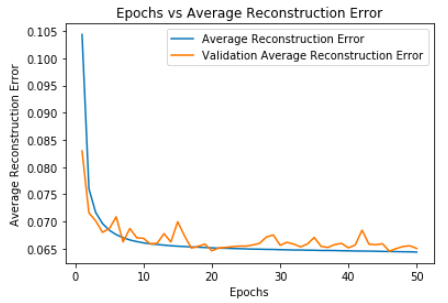
\includegraphics[width=0.35\textwidth]{4.png}
            \caption{Epochs vs Average Reconstruction Error for encoder with 1 Hidden layer with 32 Nodes}
    \end{figure}

    This encoder was then tested on the seperate test and these were the resulting metrics:

    \begin{itemize}
        \item Loss: 0.01296
        \item Average Reconstruction Error: 0.06502\\
    \end{itemize}

    Shown below is an example image and it's reconstruction from the autoencoder:

    \begin{figure}[H]
        \centering
        \captionsetup{justification=centering}
        \centering
            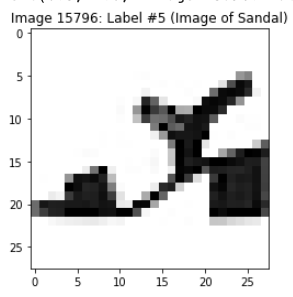
\includegraphics[width=0.15\textwidth]{5.png}
            \caption{Sample Image from Dataset}
    \end{figure}

    \begin{figure}[H]
        \centering
        \captionsetup{justification=centering}
        \centering
            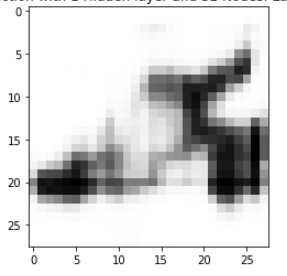
\includegraphics[width=0.15\textwidth]{6.png}
            \caption{Reconstruction from encoder with 1 Hidden layer with 32 Nodes}
    \end{figure}

    % ---------------------------------------------------- Encoder with 1 Hidden Layer that has 64 Nodes --------------------------------------------------------------------------------------------------------
    \subsection{Training Encoder with 1 Hidden Layer that has 64 Nodes}

    Shown below is the summary of the Encoder created with 1 Hidden Layer that has 64 Nodes

    \begin{figure}[H]
        \centering
        \captionsetup{justification=centering}
        \centering
            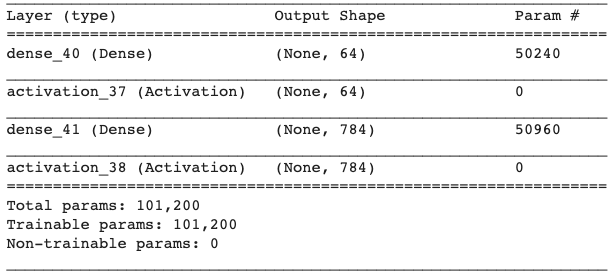
\includegraphics[width=0.45\textwidth]{7.png}
            \caption{Summary of Encoder with 1 Hidden layer with 64 Nodes}
    \end{figure}

    This encoder was trained up 50 epochs and in the end these were it's final metrics:

    \begin{itemize}
        \item Loss: 0.0089
        \item Average Reconstruction Error: 0.0523
        \item Validation Loss: 0.0091
        \item Validation Average Reconstruction Error: 0.0530
    \end{itemize}

    Shown below is the Epochs vs Loss curve for the network:

    \begin{figure}[H]
        \centering
        \captionsetup{justification=centering}
        \centering
            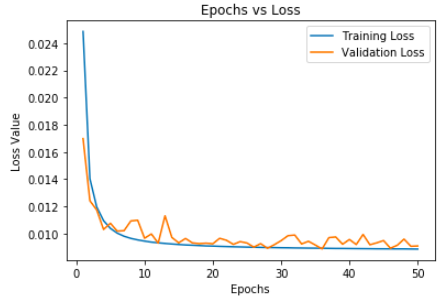
\includegraphics[width=0.35\textwidth]{8.png}
            \caption{Epochs vs Loss curve for encoder with 1 Hidden layer with 64 Nodes}
    \end{figure}

    Shown below is the Epochs vs Average reconstruction error for the network:

    \begin{figure}[H]
        \centering
        \captionsetup{justification=centering}
        \centering
            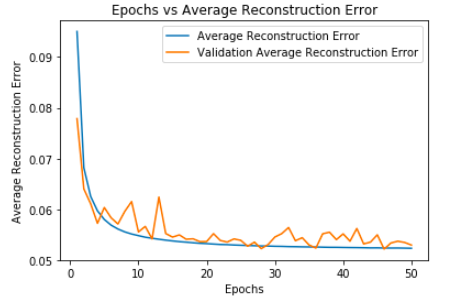
\includegraphics[width=0.35\textwidth]{9.png}
            \caption{Epochs vs Average Reconstruction Error for encoder with 1 Hidden layer with 64 Nodes}
    \end{figure}

    This encoder was then tested on the seperate test and these were the resulting metrics:

    \begin{itemize}
        \item Loss: 0.00907
        \item Average Reconstruction Error: 0.05293\\
    \end{itemize}

    Shown below is an example image and it's reconstruction from the autoencoder:

    \begin{figure}[H]
        \centering
        \captionsetup{justification=centering}
        \centering
            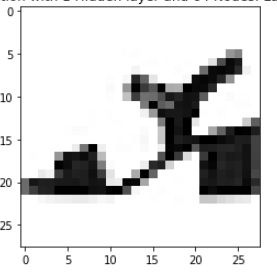
\includegraphics[width=0.15\textwidth]{10.png}
            \caption{Sample Image from Dataset}
    \end{figure}

    \begin{figure}[H]
        \centering
        \captionsetup{justification=centering}
        \centering
            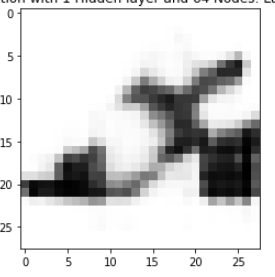
\includegraphics[width=0.15\textwidth]{11.png}
            \caption{Reconstruction from encoder with 1 Hidden layer with 64 Nodes}
    \end{figure}



    % ---------------------------------------------------- Encoder with 3 Hidden layers, main layer has 32 Nodes --------------------------------------------------------------------------------------------------------
    \subsection{Training Encoder with 3 Hidden layers, main layer has 32 Nodes}

    Shown below is the summary of the Encoder created with 3 Hidden Layers and the main one having 32 Nodes

    \begin{figure}[H]
        \centering
        \captionsetup{justification=centering}
        \centering
            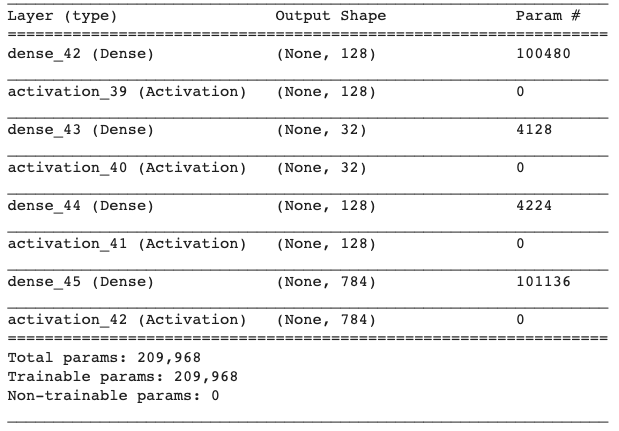
\includegraphics[width=0.45\textwidth]{12.png}
            \caption{Summary of Encoder with 3 Hidden layer and main layer having 32 Nodes}
    \end{figure}

    This encoder was trained up 50 epochs and in the end these were it's final metrics:

    \begin{itemize}
        \item Loss: 0.0098
        \item Average Reconstruction Error: 0.0513
        \item Validation Loss: 0.0099
        \item Validation Average Reconstruction Error: 0.0512
    \end{itemize}

    Shown below is the Epochs vs Loss curve for the network:

    \begin{figure}[H]
        \centering
        \captionsetup{justification=centering}
        \centering
            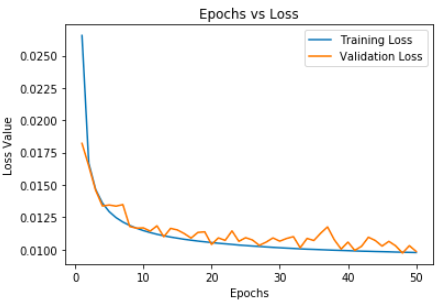
\includegraphics[width=0.35\textwidth]{13.png}
            \caption{Epochs vs Loss curve for Encoder with 3 Hidden layer and main layer having 32 Nodes}
    \end{figure}

    Shown below is the Epochs vs Average reconstruction error for the network:

    \begin{figure}[H]
        \centering
        \captionsetup{justification=centering}
        \centering
            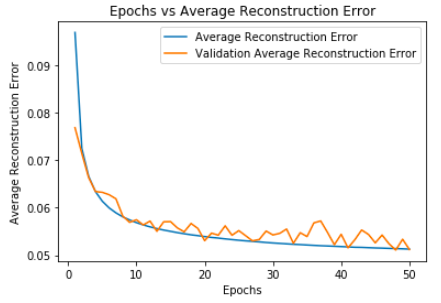
\includegraphics[width=0.35\textwidth]{14.png}
            \caption{Epochs vs Average Reconstruction Error for Encoder with 3 Hidden layer and main layer having 32 Nodes}
    \end{figure}

    This encoder was then tested on the seperate test and these were the resulting metrics:

    \begin{itemize}
        \item Loss: 0.009809
        \item Average Reconstruction Error: 0.05114\\
    \end{itemize}

    Shown below is an example image and it's reconstruction from the autoencoder:

    \begin{figure}[H]
        \centering
        \captionsetup{justification=centering}
        \centering
            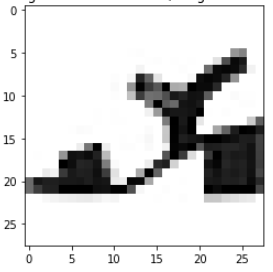
\includegraphics[width=0.15\textwidth]{15.png}
            \caption{Sample Image from Dataset}
    \end{figure}

    \begin{figure}[H]
        \centering
        \captionsetup{justification=centering}
        \centering
            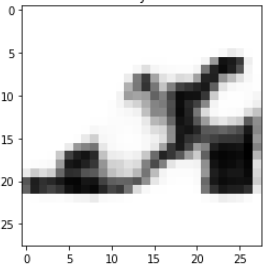
\includegraphics[width=0.15\textwidth]{16.png}
            \caption{Reconstruction from Encoder with 3 Hidden layer and main layer having 32 Nodes}
    \end{figure}

    % ---------------------------------------------------- Encoder with 3 Hidden layers, main layer has 64 Nodes --------------------------------------------------------------------------------------------------------
    \subsection{Training Encoder with 3 Hidden layers, main layer has 64 Nodes}

    Shown below is the summary of the Encoder created with 3 Hidden Layers and the main one having 64 Nodes

    \begin{figure}[H]
        \centering
        \captionsetup{justification=centering}
        \centering
            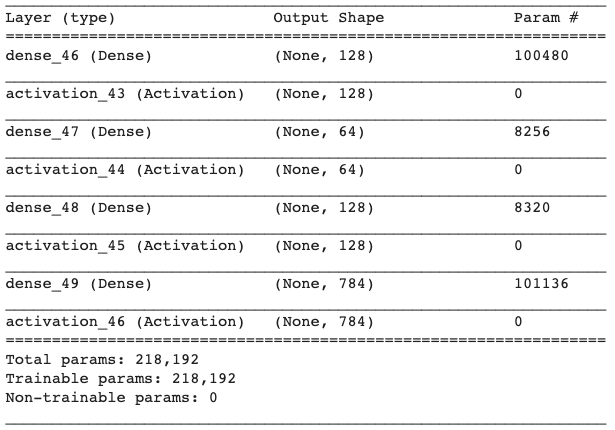
\includegraphics[width=0.45\textwidth]{17.png}
            \caption{Summary of Encoder with 3 Hidden layer and main layer having 64 Nodes}
    \end{figure}

    This encoder was trained up 50 epochs and in the end these were it's final metrics:

    \begin{itemize}
        \item Loss: 0.0083
        \item Average Reconstruction Error: 0.0481 
        \item Validation Loss: 0.0083
        \item Validation Average Reconstruction Error: 0.0485
    \end{itemize}

    Shown below is the Epochs vs Loss curve for the network:

    \begin{figure}[H]
        \centering
        \captionsetup{justification=centering}
        \centering
            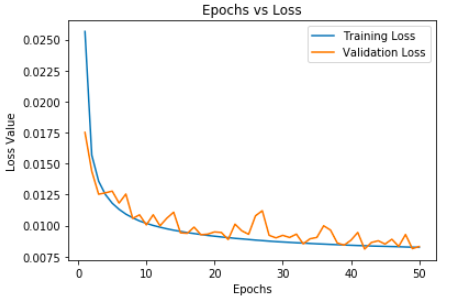
\includegraphics[width=0.35\textwidth]{18.png}
            \caption{Epochs vs Loss curve for Encoder with 3 Hidden layer and main layer having 64 Nodes}
    \end{figure}

    Shown below is the Epochs vs Average reconstruction error for the network:

    \begin{figure}[H]
        \centering
        \captionsetup{justification=centering}
        \centering
            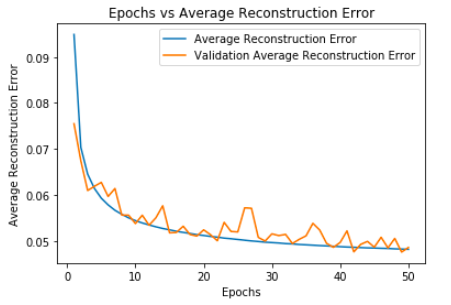
\includegraphics[width=0.35\textwidth]{19.png}
            \caption{Epochs vs Average Reconstruction Error for Encoder with 3 Hidden layer and main layer having 64 Nodes}
    \end{figure}

    This encoder was then tested on the seperate test and these were the resulting metrics:

    \begin{itemize}
        \item Loss: 0.00829
        \item Average Reconstruction Error: 0.0484\\
    \end{itemize}

    Shown below is an example image and it's reconstruction from the autoencoder:

    \begin{figure}[H]
        \centering
        \captionsetup{justification=centering}
        \centering
            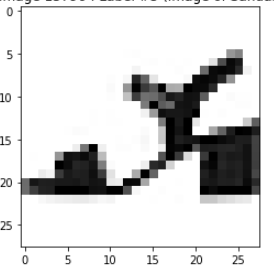
\includegraphics[width=0.15\textwidth]{20.png}
            \caption{Sample Image from Dataset}
    \end{figure}

    \begin{figure}[H]
        \centering
        \captionsetup{justification=centering}
        \centering
            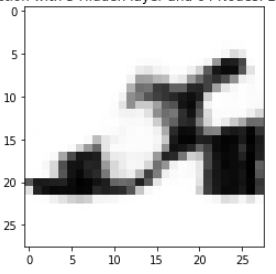
\includegraphics[width=0.15\textwidth]{21.png}
            \caption{Reconstruction from Encoder with 3 Hidden layer and main layer having 64 Nodes}
    \end{figure}

    \subsection{Comments}

    The multiple layer Encoders outperform the single layer encoders. The network with 3 hidden layers and
    64 nodes in the center is the best performing one out of all. The order of worst performing to best is from A, B, C to D. 

    \section{Denoising autoencoders}

    Here I use the same data as in Task 1 for training and testing.
    However, before applying as input I corrupt the images with 0 mean additive gaussian noise with
    some standard deviation value. I change the noise standard deviation level to 0.1, 0.2 and 0.3. 
    While showing a few reconstructed examples along with the corresponding noisy images.
    Then I comment on the quality and report the root mean square error between the reconstructed testing images and clean testing images for the three noise levels
    and the two architectures with different dimensionality of the representative codes.

    \subsection{Preprocessing}

    Noise was added using numpys random.normal function which let use add noise with different standard deviation to each image.
    Shown below is the original image along with the image corrupted with noise of standard deviation 0.1, 0.2 and 0.3.
    
    \begin{figure}[H]
        \centering
        \captionsetup{justification=centering}
        \centering
            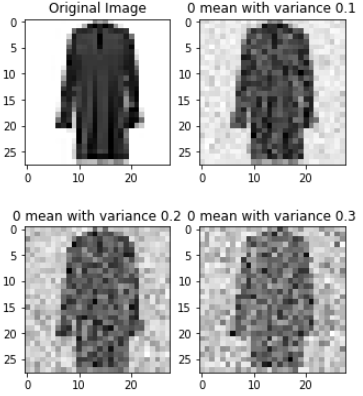
\includegraphics[width=0.2\textwidth]{22.png}
            \caption{Original image and image corrupted with different noise variances}
    \end{figure}

    \subsection{32 node convolutional autoencoder}

    A convolutional autoencoder was implemented and it's architecture can be seen below:

    \begin{figure}[H]
        \centering
        \captionsetup{justification=centering}
        \centering
            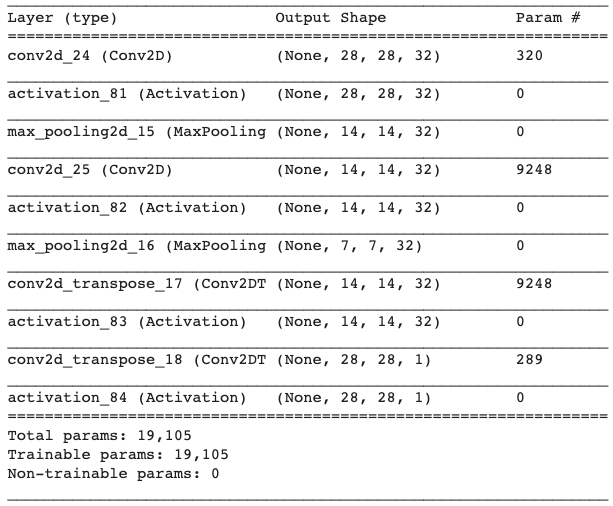
\includegraphics[width=0.45\textwidth]{23.png}
            \caption{32 node convolutional autoencoder architecture}
    \end{figure}

    \subsubsection{Training on 0.1 variance and 0 mean noise\\}

    This denoising autoencoder was trained with 65 epochs on the noisy data with the clean data as output label. Shown below
    are its metrics after training:

    \begin{itemize}
        \item Loss: 0.0036
        \item Average Reconstruction Error: 0.0315
        \item Validation Loss: 0.0037
        \item Validation Average Reconstruction Error: 0.0318
    \end{itemize}

    Shown below is the Epochs vs Loss curve for the denoising autoencoder:

    \begin{figure}[H]
        \centering
        \captionsetup{justification=centering}
        \centering
            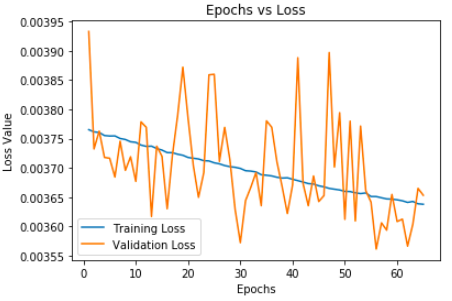
\includegraphics[width=0.35\textwidth]{24.png}
            \caption{Epochs vs Loss curve for 32 node convolutional autoencoder}
    \end{figure}

    Shown below is the Epochs vs Average reconstruction error for the denoising autoencoder:

    \begin{figure}[H]
        \centering
        \captionsetup{justification=centering}
        \centering
            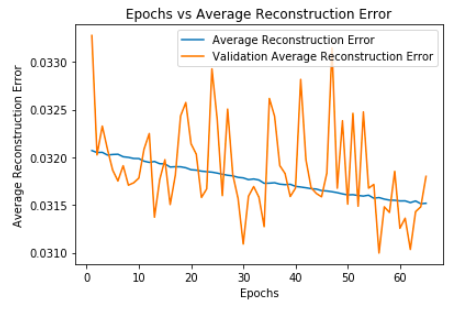
\includegraphics[width=0.35\textwidth]{25.png}
            \caption{Epochs vs Average Reconstruction Error for 32 node convolutional autoencoder}
    \end{figure}

    This autoencoder was then tested on the seperate test and these were the resulting metrics:

    \begin{itemize}
        \item Loss: 0.003687
        \item Average Reconstruction Error: 0.03192\\
    \end{itemize}

    Shown below is an example image, noisy image and it's reconstruction from the autoencoder:

    \begin{figure}[H]
        \centering
        \captionsetup{justification=centering}
        \centering
            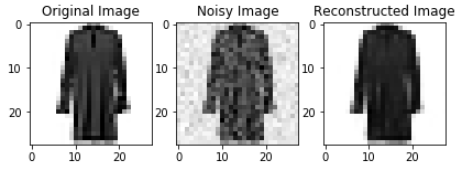
\includegraphics[width=0.4\textwidth]{26.png}
            \caption{Image, noisy image (0.1) and it's reconstruction from the denoising autoencoder with 32 nodes}
    \end{figure}




    \subsubsection{Training on 0.2 variance and 0 mean noise\\}

    This denoising autoencoder was trained with 65 epochs on the noisy data with the clean data as output label. Shown below
    are its metrics after training:

    \begin{itemize}
        \item Loss: 0.0060
        \item Average Reconstruction Error: 0.0413
        \item Validation Loss: 0.0060 
        \item Validation Average Reconstruction Error: 0.0413
    \end{itemize}

    Shown below is the Epochs vs Loss curve for the denoising autoencoder:

    \begin{figure}[H]
        \centering
        \captionsetup{justification=centering}
        \centering
            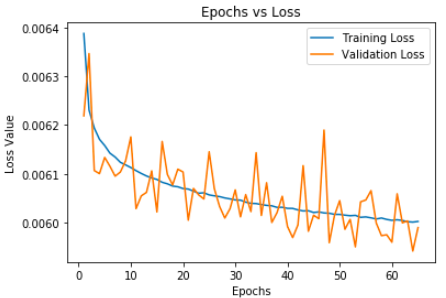
\includegraphics[width=0.35\textwidth]{27.png}
            \caption{Epochs vs Loss curve for 32 node convolutional autoencoder}
    \end{figure}

    Shown below is the Epochs vs Average reconstruction error for the denoising autoencoder:

    \begin{figure}[H]
        \centering
        \captionsetup{justification=centering}
        \centering
            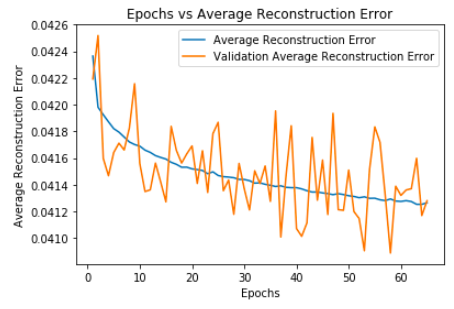
\includegraphics[width=0.35\textwidth]{28.png}
            \caption{Epochs vs Average Reconstruction Error for 32 node convolutional autoencoder}
    \end{figure}

    This autoencoder was then tested on the seperate test and these were the resulting metrics:

    \begin{itemize}
        \item Loss: 0.006031
        \item Average Reconstruction Error: 0.04141\\
    \end{itemize}

    Shown below is an example image, noisy image and it's reconstruction from the autoencoder:

    \begin{figure}[H]
        \centering
        \captionsetup{justification=centering}
        \centering
            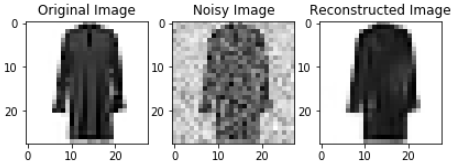
\includegraphics[width=0.4\textwidth]{29.png}
            \caption{Image, noisy image (0.2) and it's reconstruction from the denoising autoencoder with 32 nodes}
    \end{figure}




    \subsubsection{Training on 0.3 variance and 0 mean noise\\}

    This denoising autoencoder was trained with 65 epochs on the noisy data with the clean data as output label. Shown below
    are its metrics after training:

    \begin{itemize}
        \item Loss: 0.0089
        \item Average Reconstruction Error: 0.0511
        \item Validation Loss: 0.0091
        \item Validation Average Reconstruction Error: 0.0516
    \end{itemize}

    Shown below is the Epochs vs Loss curve for the denoising autoencoder:

    \begin{figure}[H]
        \centering
        \captionsetup{justification=centering}
        \centering
            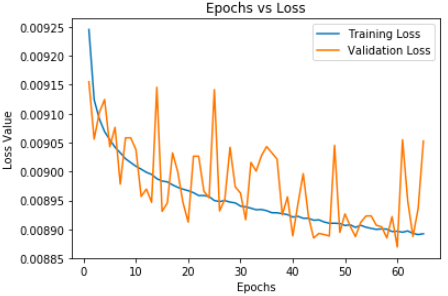
\includegraphics[width=0.35\textwidth]{30.png}
            \caption{Epochs vs Loss curve for 32 node convolutional autoencoder}
    \end{figure}

    Shown below is the Epochs vs Average reconstruction error for the denoising autoencoder:

    \begin{figure}[H]
        \centering
        \captionsetup{justification=centering}
        \centering
            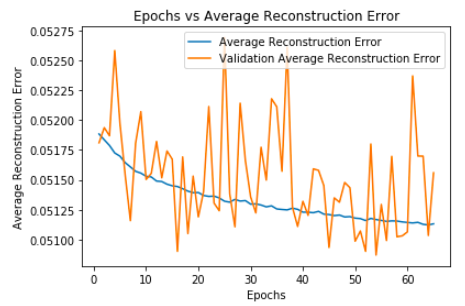
\includegraphics[width=0.35\textwidth]{31.png}
            \caption{Epochs vs Average Reconstruction Error for 32 node convolutional autoencoder}
    \end{figure}

    This autoencoder was then tested on the seperate test and these were the resulting metrics:

    \begin{itemize}
        \item Loss: 0.009111
        \item Average Reconstruction Error: 0.05177\\
    \end{itemize}

    Shown below is an example image, noisy image and it's reconstruction from the autoencoder:

    \begin{figure}[H]
        \centering
        \captionsetup{justification=centering}
        \centering
            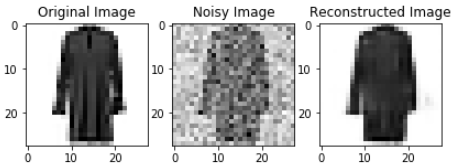
\includegraphics[width=0.4\textwidth]{32.png}
            \caption{Image, noisy image (0.3) and it's reconstruction from the denoising autoencoder with 32 nodes}
    \end{figure}













    \subsection{64 node convolutional autoencoder}

    A convolutional autoencoder was implemented and it's architecture can be seen below:

    \begin{figure}[H]
        \centering
        \captionsetup{justification=centering}
        \centering
            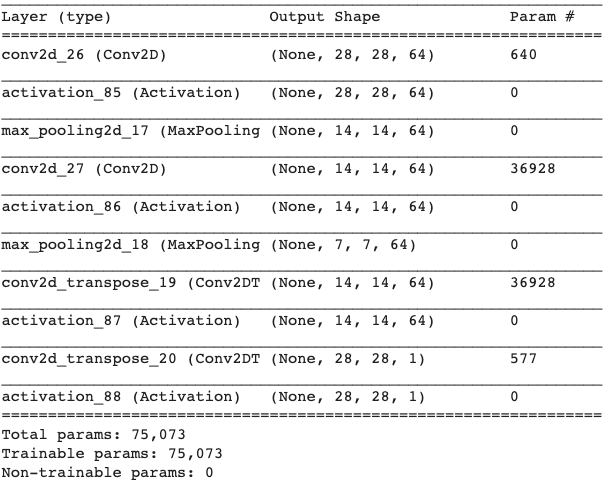
\includegraphics[width=0.45\textwidth]{33.png}
            \caption{64 node convolutional autoencoder architecture}
    \end{figure}

    \subsubsection{Training on 0.1 variance and 0 mean noise\\}

    This denoising autoencoder was trained with 65 epochs on the noisy data with the clean data as output label. Shown below
    are its metrics after training:

    \begin{itemize}
        \item Loss: 0.0030
        \item Average Reconstruction Error: 0.0288
        \item Validation Loss: 0.0031
        \item Validation Average Reconstruction Error: 0.0293
    \end{itemize}

    Shown below is the Epochs vs Loss curve for the denoising autoencoder:

    \begin{figure}[H]
        \centering
        \captionsetup{justification=centering}
        \centering
            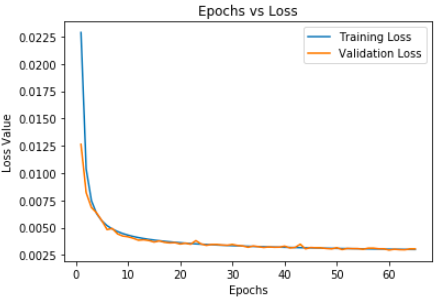
\includegraphics[width=0.35\textwidth]{34.png}
            \caption{Epochs vs Loss curve for 64 node convolutional autoencoder}
    \end{figure}

    Shown below is the Epochs vs Average reconstruction error for the denoising autoencoder:

    \begin{figure}[H]
        \centering
        \captionsetup{justification=centering}
        \centering
            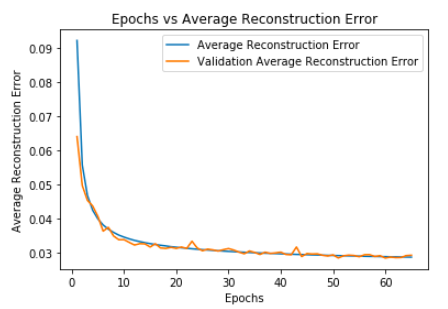
\includegraphics[width=0.35\textwidth]{35.png}
            \caption{Epochs vs Average Reconstruction Error for 64 node convolutional autoencoder}
    \end{figure}

    This autoencoder was then tested on the seperate test and these were the resulting metrics:

    \begin{itemize}
        \item Loss: 0.0030992
        \item Average Reconstruction Error: 0.029463\\
    \end{itemize}

    Shown below is an example image, noisy image and it's reconstruction from the autoencoder:

    \begin{figure}[H]
        \centering
        \captionsetup{justification=centering}
        \centering
            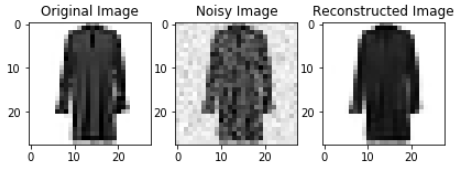
\includegraphics[width=0.4\textwidth]{36.png}
            \caption{Image, noisy image (0.1) and it's reconstruction from the denoising autoencoder with 64 nodes}
    \end{figure}




    \subsubsection{Training on 0.2 variance and 0 mean noise\\}

    This denoising autoencoder was trained with 65 epochs on the noisy data with the clean data as output label. Shown below
    are its metrics after training: 

    \begin{itemize}
        \item Loss: 0.0053
        \item Average Reconstruction Error: 0.0384
        \item Validation Loss: 0.0054
        \item Validation Average Reconstruction Error: 0.0392
    \end{itemize}

    Shown below is the Epochs vs Loss curve for the denoising autoencoder:

    \begin{figure}[H]
        \centering
        \captionsetup{justification=centering}
        \centering
            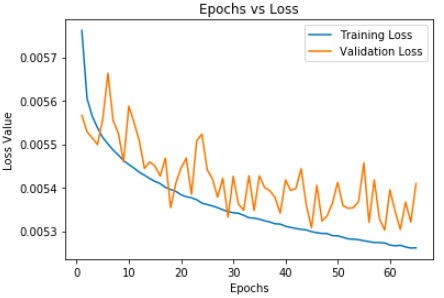
\includegraphics[width=0.35\textwidth]{37.png}
            \caption{Epochs vs Loss curve for 64 node convolutional autoencoder}
    \end{figure}

    Shown below is the Epochs vs Average reconstruction error for the denoising autoencoder:

    \begin{figure}[H]
        \centering
        \captionsetup{justification=centering}
        \centering
            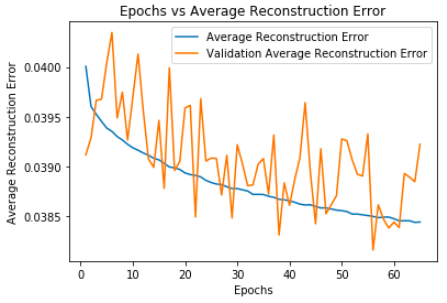
\includegraphics[width=0.35\textwidth]{38.png}
            \caption{Epochs vs Average Reconstruction Error for 64 node convolutional autoencoder}
    \end{figure}

    This autoencoder was then tested on the seperate test and these were the resulting metrics:

    \begin{itemize}
        \item Loss: 0.005457
        \item Average Reconstruction Error: 0.03937\\
    \end{itemize}

    Shown below is an example image, noisy image and it's reconstruction from the autoencoder:

    \begin{figure}[H]
        \centering
        \captionsetup{justification=centering}
        \centering
            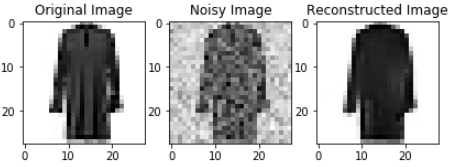
\includegraphics[width=0.4\textwidth]{39.png}
            \caption{Image, noisy image (0.2) and it's reconstruction from the denoising autoencoder with 64 nodes}
    \end{figure}




    \subsubsection{Training on 0.3 variance and 0 mean noise\\}

    This denoising autoencoder was trained with 65 epochs on the noisy data with the clean data as output label. Shown below
    are its metrics after training:

    \begin{itemize}
        \item Loss: 0.0080
        \item Average Reconstruction Error: 0.0481
        \item Validation Loss: 0.0082
        \item Validation Average Reconstruction Error: 0.0490
    \end{itemize}

    Shown below is the Epochs vs Loss curve for the denoising autoencoder:

    \begin{figure}[H]
        \centering
        \captionsetup{justification=centering}
        \centering
            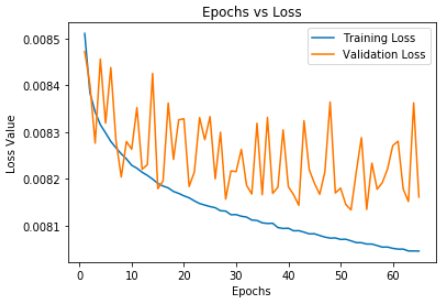
\includegraphics[width=0.35\textwidth]{40.png}
            \caption{Epochs vs Loss curve for 64 node convolutional autoencoder}
    \end{figure}

    Shown below is the Epochs vs Average reconstruction error for the denoising autoencoder:

    \begin{figure}[H]
        \centering
        \captionsetup{justification=centering}
        \centering
            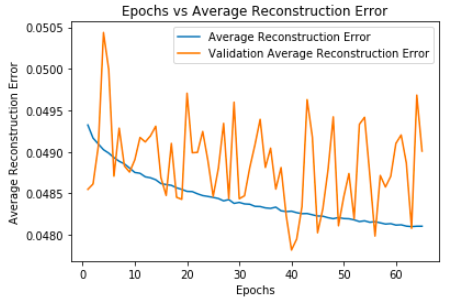
\includegraphics[width=0.35\textwidth]{41.png}
            \caption{Epochs vs Average Reconstruction Error for 64 node convolutional autoencoder}
    \end{figure}

    This autoencoder was then tested on the seperate test and these were the resulting metrics:

    \begin{itemize}
        \item Loss: 0.008227
        \item Average Reconstruction Error: 0.04924\\
    \end{itemize}

    Shown below is an example image, noisy image and it's reconstruction from the autoencoder:

    \begin{figure}[H]
        \centering
        \captionsetup{justification=centering}
        \centering
            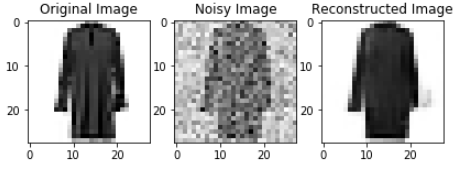
\includegraphics[width=0.4\textwidth]{42.png}
            \caption{Image, noisy image (0.3) and it's reconstruction from the denoising autoencoder with 64 nodes}
    \end{figure}

    \subsection{Comments}

    In all cases the 64 node denoising autoencoder outperforms the 32 node one. The individual performances are visible in
    each of the subsections above. While the quality is almost identical the autoencoder does tend to loose certain elements
    of shading across the data and in high noise image there are artifacts produced.

    \section{LSTM networks}

    Data is given that is sequences of accelerometer and gyroscope data from an IMU attached
    to the shoe of three subjects. The subjects are asked to walk/run on a treadmill at 12 different speeds.

    Using the data for subject 1 as training and the data for subject 2 as validation and building my own LSTM network.
    I picked the structure that gives you the best performance with the hardware available from Google Collab. Then I combineed 
    the data for subject 1 and subject 2 and used it to train a network that was tested on data from subject 4. Also reported the average
    root mean squated error for speed estimation, both on the training data and testing data.

    \subsection{Preprocessing}

    Data was uploaded to Google Drive and then imported from there. This was done so that no data was lost due to incomplete upload
    or lost through a runtime disconnection on Google Collab. The size of the data was as follows:

    \begin{itemize}
        \item Size of Subject data is (12000, 600, 6)
        \item Size of Truth data is (12000, 1)
    \end{itemize} 

    \subsection{Training with Subject 1 and Validating with Subject 2}

    A LSTM network was written in Keras and it's architecture is shown below, mean squared error was the loss function.

    \begin{figure}[H]
        \centering
        \captionsetup{justification=centering}
        \centering
            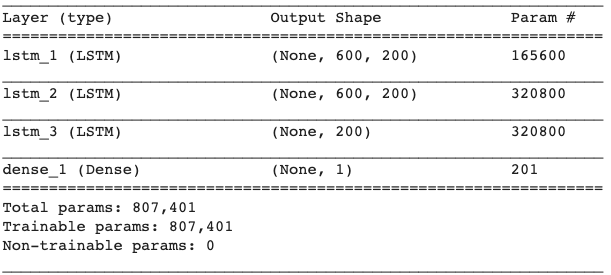
\includegraphics[width=0.45\textwidth]{43.png}
            \caption{Architecture of LSTM network}
    \end{figure}

    Training of the network was only done on 3 epochs with a batch size of 148. This is because Google collab would crash due to RAM limitations on
    higher epochs. The final learning metrics are:

    \begin{itemize}
        \item Loss: 0.0918
        \item Accuracy: 0.4565
        \item Validation Loss: 1.7333
        \item Validation Accuracy: 0.1515
    \end{itemize}

    Shown below is the loss and accuracy vs those 3 epochs.
    
    \begin{figure}[H]
        \centering
        \captionsetup{justification=centering}
        \centering
            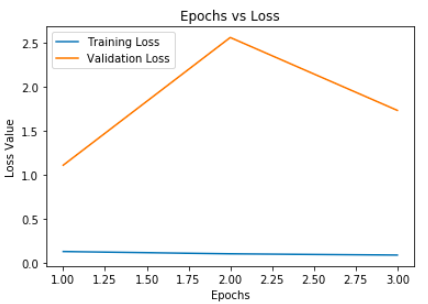
\includegraphics[width=0.35\textwidth]{44.png}
            \caption{Epochs vs Loss}
    \end{figure}

    \begin{figure}[H]
        \centering
        \captionsetup{justification=centering}
        \centering
            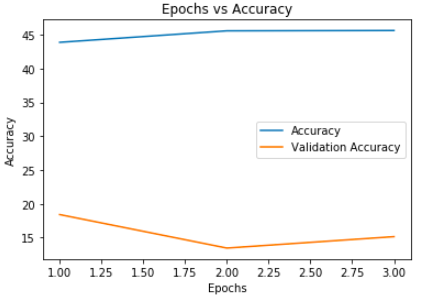
\includegraphics[width=0.35\textwidth]{45.png}
            \caption{Epochs vs Accuracy}
    \end{figure}

    \section{Training with Subject 1 and 2, Testing on Subject 4}

    The data of subject 1 and 2 was first concatenated and therefore the data shapes were as follows:

    \begin{itemize}
        \item Size of Subject 1 and 2 mixed data is (24000, 600, 6)
        \item Size of Subject 4 data is (12000, 600, 6)
        \item Size of Subject 1 and 2 mixed truth data is (12000, 1)
        \item Size of Subject 4 truth data is (12000, 1)
    \end{itemize} 

    The mixed data was then input the same network as in figure 43 and it was trained once again over 3 epochs due to limitations on Google
    collab. The final learning metrics are:

    \begin{itemize}
        \item Loss: 0.1852
        \item Accuracy: 0.4003
    \end{itemize}

    Shown below is the loss and accuracy vs those 3 epochs.
    
    \begin{figure}[H]
        \centering
        \captionsetup{justification=centering}
        \centering
            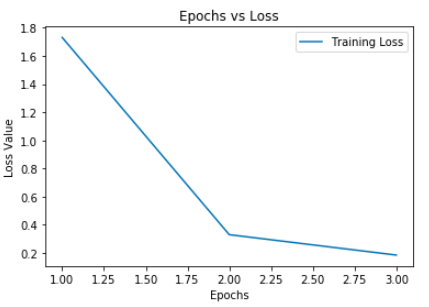
\includegraphics[width=0.35\textwidth]{46.png}
            \caption{Epochs vs Loss}
    \end{figure}

    \begin{figure}[H]
        \centering
        \captionsetup{justification=centering}
        \centering
            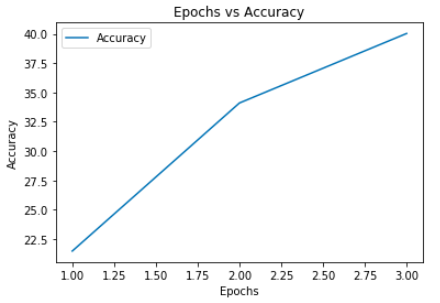
\includegraphics[width=0.35\textwidth]{47.png}
            \caption{Epochs vs Accuracy}
    \end{figure}

    The data was then tested using subject 4s data and the results were as follows:

    \begin{itemize}
        \item Loss: 2.588
        \item Accuracy: 0.11099
    \end{itemize}


    \section{Variational Autoencoders}

    Using regular autoencoders one of the main limitations is that the the latent space it converts inputs to is not always continuous. This means we cannot easily interpolate between different points of the latent space. This means if we randomly sample from the latent space we do not always get some meaningful variation of an input image and therefore using an decoder means we cannot truly generate new or interpolated data by sampling. Variational autoencoders solve this and allow for generative modelling because the latent spaces they map to are always continous and can easily be sampled. To do this the encoder outputs a mean and standard deviation for a gaussian distributed variable, so the decoder now does not get a fixed value but instead it samples a gaussian distributed region. The decoder then samples this region for points when decoding and this teaches it that a specific point is not referring to a sample of a class but instead the entire region corresponds to a class. Through training the decoder learns the mean and standard deviations but it may place classes far apart in the latent space even though they may be close to each other. To prevent it from doing this the loss function also includes the KL divergence which is a measure of how much two distributions diverge from each other so by forcing the network to minimize the loss function we can also force it to minimize the KL divergence and keep the different class distributions close to each other. The loss function also contains a reconstruction loss that ensures the the sampled data is reconstructed to the original input.

    \begin{figure}[H]
        \centering
        \captionsetup{justification=centering}
        \centering
            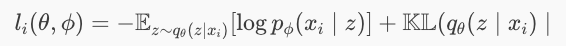
\includegraphics[width=0.35\textwidth]{48.png}
            \caption{Loss Function of Variational Autoencoders}
    \end{figure}

\end{document}